In this report, we design two structured products on a single underlying, the stock of \gls{jpm}, which is listed on the New York Stock Exchange and traded in U.S.\ dollars (USD).
The first product is a \gls{pppn}, the second an Airbag Note.
For each product, we describe the payoff, replicate it with a zero-coupon bond and European options using real market prices, and estimate its expected performance with a Monte Carlo simulation.
All computations and figures can be reproduced with the accompanying Python notebook.

\subsection{Market Data}
All market data was collected from Yahoo Finance\footnote{\url{https://finance.yahoo.com/quote/JPM/}} on November 12, 2025, at 12:00 PM Eastern Time, during regular U.S.\ trading hours.
We take this moment as $t = 0$.
The snapshot contains the spot price of \gls{jpm}, $S_0 = 320.41$, and the full option chain for the maturity date of January 15, 2027.
All prices and payoffs in this report are expressed in USD.

\paragraph{Risk-Free Rate}
The time from November 12, 2025, to January 15, 2027, is 14 months, so $T = \frac{14}{12} \approx 1.167$.
For the risk-free rate $r$, we take the 1-year and 2-year U.S.\ Treasury par yields on November 12, 2025 ($3.65\%$ and $3.56\%$) and interpolate linearly to 14 months, which gives $r = 3.635\%$.
We assume this rate to be constant and continuously compounded throughout the report.

\paragraph{Option Data}
On November 12, 2025, the market quoted $47$ European calls and $41$ European puts on \gls{jpm}, all maturing on January 15, 2027, with strikes between $105$ and $470$.
Some strikes are not quoted for puts, which explains the smaller number of puts.
Fig.~\ref{fig:option-prices} shows the quoted prices over the strike range.

\begin{figure}[h]
    \centering
    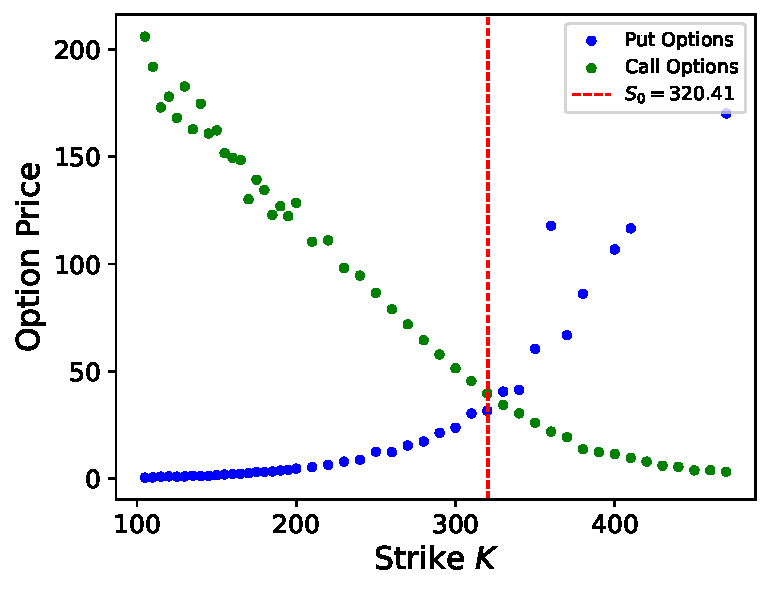
\includegraphics[width=0.5\linewidth]{option_prices.pdf}
    \caption{\textbf{Option Prices.} Market prices of the European puts and calls on \gls{jpm} with maturity January 15, 2027, quoted on November 12, 2025.}
    \label{fig:option-prices}
\end{figure}
